%----------------------------------------
% DÉCOMPOSITION AGENT-ENVIRONEMENT
%----------------------------------------

\begin{frame}{Environnement}{Décomposition}
\begin{itemize}
\item Séparation entre l'agent et son environment.
\item Configurations quelconques d'agents sont possibles.
\end{itemize}
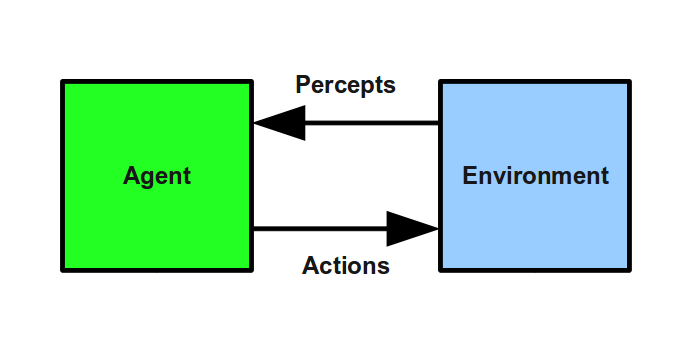
\includegraphics[width=\textwidth]{img/env_sim/agent_env}\\
\end{frame}

%----------------------------------------
% ARBITRE
%----------------------------------------

\begin{frame}{Environnement}{Arbitre}
\begin{itemize}
\item L'environment est assimilé à un arbitre.
\item L'agent-joueur interagit avec celui-ci de manière asynchrone.
\end{itemize}
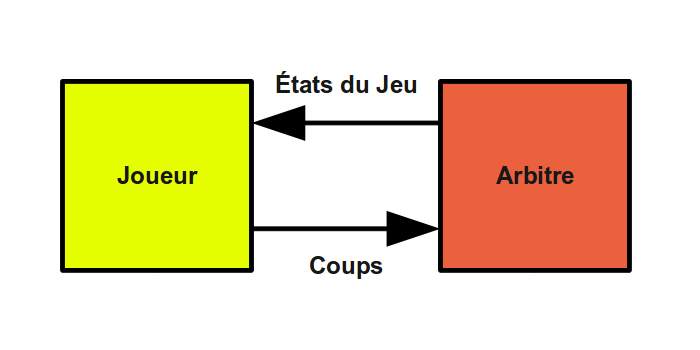
\includegraphics[width=\textwidth]{img/env_sim/agent_arb}\\
\end{frame}


%----------------------------------------
% WEBSERVICE "GAME SERVICE"
%----------------------------------------

\begin{frame}{Environnement}{Webservice \texttt{game\_service}}

\begin{block}{Serveur: Servlets Java}
\begin{itemize}
\item Classe Java instancié pour chaque requète HTTP.
\item Répond avec un XML représentative d'état (REST).
\end{itemize}
\end{block}

\pause

\begin{block}{Client: Page HTML 5}
\begin{itemize}
\item Maintient l'état du jeu par polling (jQuery / AJAX).
\item Réponses asynchrones traités par callback.
\end{itemize}
\end{block}


\end{frame}


%----------------------------------------
% RULEBOOK
%----------------------------------------

\begin{frame}{Simulation}{Rulebook}

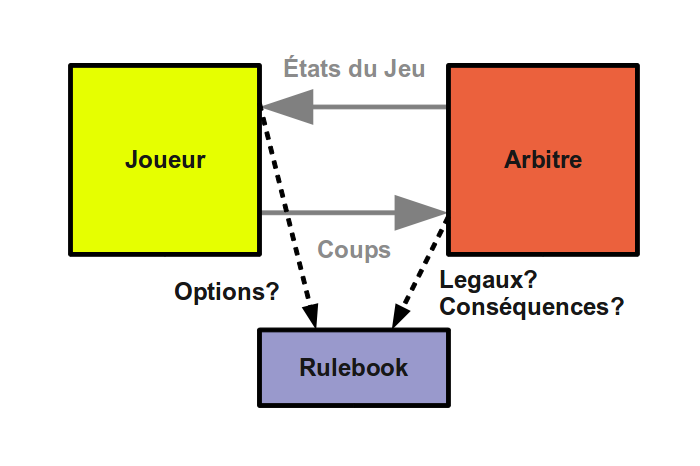
\includegraphics[width=\textwidth]{img/env_sim/rulebook}

\end{frame}


%----------------------------------------
% LIBRARIE "GAME LOGIC"
%----------------------------------------

\begin{frame}{Simulation}{Bibliothèque \texttt{game\_logic}}

\begin{block}{Classe \texttt{BoardMatrix}}
Plateau sous forme matricielle avec accesseurs adaptés.
\end{block}

\pause

\begin{block}{Classe abstraite \texttt{Rules}}
\begin{itemize}
\item Forme du plateau? Configuration initiale?
\item Qui joue en premier?
\item Quand a-t-on gagné? Perdu? Un match nul?
\item Quelles sont les coups possibles?
\end{itemize}
\end{block}

\pause

\begin{block}{Classe \texttt{Game}}
Associe un \texttt{Rules}, un \texttt{BoardMatrix}, un état, un joueur courant...
\end{block}

\end{frame}